\documentclass{standalone}
\usepackage{tikz}
\usetikzlibrary{patterns, positioning}

\begin{document}
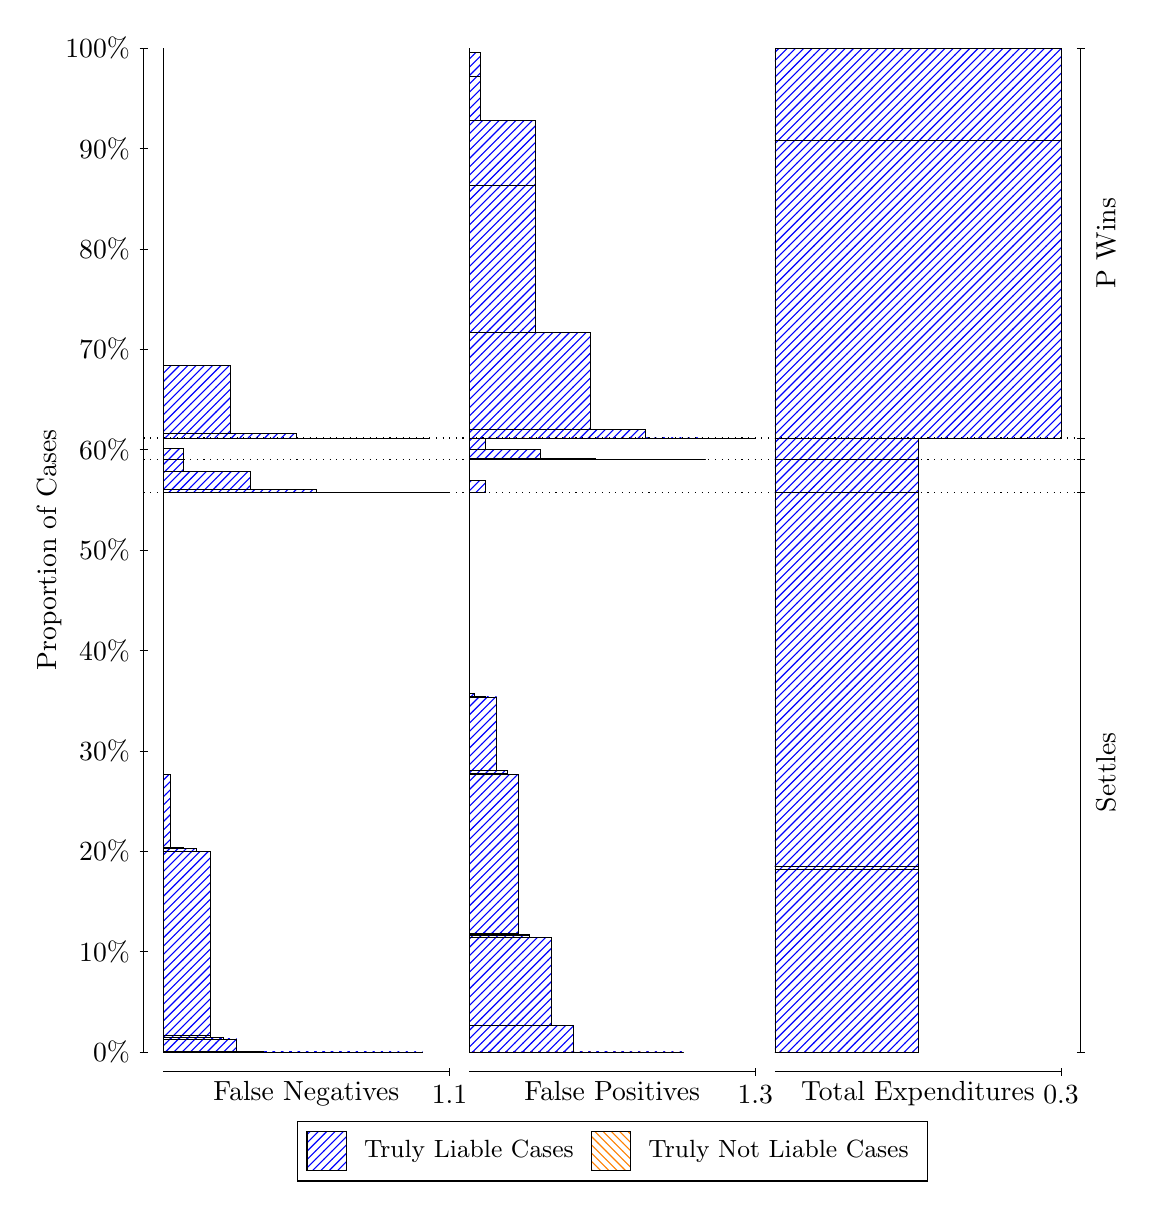
\begin{tikzpicture}
\draw[black, very thin] (1.5,1.75) -- (1.5,14.5);
\node[rotate=90, anchor=center] at (0.3, 8.125) {Proportion of Cases};
\draw[black, very thin] (1.45,1.75) -- (1.55,1.75);
\node[anchor=east] at (1.45, 1.75) {0\%};
\draw[black, very thin] (1.45,3.025) -- (1.55,3.025);
\node[anchor=east] at (1.45, 3.025) {10\%};
\draw[black, very thin] (1.45,4.3) -- (1.55,4.3);
\node[anchor=east] at (1.45, 4.3) {20\%};
\draw[black, very thin] (1.45,5.575) -- (1.55,5.575);
\node[anchor=east] at (1.45, 5.575) {30\%};
\draw[black, very thin] (1.45,6.85) -- (1.55,6.85);
\node[anchor=east] at (1.45, 6.85) {40\%};
\draw[black, very thin] (1.45,8.125) -- (1.55,8.125);
\node[anchor=east] at (1.45, 8.125) {50\%};
\draw[black, very thin] (1.45,9.4) -- (1.55,9.4);
\node[anchor=east] at (1.45, 9.4) {60\%};
\draw[black, very thin] (1.45,10.675) -- (1.55,10.675);
\node[anchor=east] at (1.45, 10.675) {70\%};
\draw[black, very thin] (1.45,11.95) -- (1.55,11.95);
\node[anchor=east] at (1.45, 11.95) {80\%};
\draw[black, very thin] (1.45,13.225) -- (1.55,13.225);
\node[anchor=east] at (1.45, 13.225) {90\%};
\draw[black, very thin] (1.45,14.5) -- (1.55,14.5);
\node[anchor=east] at (1.45, 14.5) {100\%};

\draw[black, very thin] (13.4,1.75) -- (13.4,14.5);
\draw[black, very thin] (13.35,1.75) -- (13.45,1.75);
\node[anchor=west] at (13.35, 1.75) {};
\draw[black, very thin] (13.35,8.8549) -- (13.45,8.8549);
\node[anchor=west] at (13.35, 8.8549) {};
\draw[black, very thin] (13.35,9.2724) -- (13.45,9.2724);
\node[anchor=west] at (13.35, 9.2724) {};
\draw[black, very thin] (13.35,9.5471) -- (13.45,9.5471);
\node[anchor=west] at (13.35, 9.5471) {};
\draw[black, very thin] (13.35,14.5) -- (13.45,14.5);
\node[anchor=west] at (13.35, 14.5) {};

\draw[black, very thin, pattern color=blue, pattern=north east lines] (1.75,1.75) rectangle (5.0453,1.75);
\draw[black, very thin, pattern color=blue, pattern=north east lines] (1.75,1.75) rectangle (4.7074,1.75);
\draw[black, very thin, pattern color=blue, pattern=north east lines] (1.75,1.75) rectangle (4.3694,1.75);
\draw[black, very thin, pattern color=blue, pattern=north east lines] (1.75,1.75) rectangle (4.2004,1.75);
\draw[black, very thin, pattern color=blue, pattern=north east lines] (1.75,1.75) rectangle (4.0314,1.75);
\draw[black, very thin, pattern color=blue, pattern=north east lines] (1.75,1.75) rectangle (3.8624,1.75);
\draw[black, very thin, pattern color=blue, pattern=north east lines] (1.75,1.75) rectangle (3.6934,1.75);
\draw[black, very thin, pattern color=blue, pattern=north east lines] (1.75,1.75) rectangle (3.5244,1.7503);
\draw[black, very thin, pattern color=blue, pattern=north east lines] (1.75,1.7503) rectangle (3.3554,1.7522);
\draw[black, very thin, pattern color=blue, pattern=north east lines] (1.75,1.7522) rectangle (3.1864,1.7522);
\draw[black, very thin, pattern color=blue, pattern=north east lines] (1.75,1.7522) rectangle (3.1864,1.7523);
\draw[black, very thin, pattern color=blue, pattern=north east lines] (1.75,1.7523) rectangle (3.0174,1.7594);
\draw[black, very thin, pattern color=blue, pattern=north east lines] (1.75,1.7594) rectangle (2.8484,1.7595);
\draw[black, very thin, pattern color=blue, pattern=north east lines] (1.75,1.7595) rectangle (2.6795,1.9176);
\draw[black, very thin, pattern color=blue, pattern=north east lines] (1.75,1.9176) rectangle (2.6795,1.9176);
\draw[black, very thin, pattern color=blue, pattern=north east lines] (1.75,1.9176) rectangle (2.5105,1.9363);
\draw[black, very thin, pattern color=blue, pattern=north east lines] (1.75,1.9363) rectangle (2.3415,1.9363);
\draw[black, very thin, pattern color=blue, pattern=north east lines] (1.75,1.9363) rectangle (2.3415,1.956);
\draw[black, very thin, pattern color=blue, pattern=north east lines] (1.75,1.956) rectangle (2.3415,4.3015);
\draw[black, very thin, pattern color=blue, pattern=north east lines] (1.75,4.3015) rectangle (2.1725,4.3387);
\draw[black, very thin, pattern color=blue, pattern=north east lines] (1.75,4.3387) rectangle (2.0035,4.3444);
\draw[black, very thin, pattern color=blue, pattern=north east lines] (1.75,4.3444) rectangle (1.8345,5.2738);
\draw[black, very thin, pattern color=blue, pattern=north east lines] (1.75,5.2738) rectangle (1.8345,5.2739);
\draw[black, very thin, pattern color=orange, pattern=north west lines] (1.75,5.2739) rectangle (1.75,5.2739);
\draw[black, very thin, pattern color=blue, pattern=north east lines] (1.75,5.2739) rectangle (1.75,8.8549);
\draw[black, very thin, pattern color=blue, pattern=north east lines] (1.75,8.8549) rectangle (5.3833,8.8549);
\draw[black, very thin, pattern color=blue, pattern=north east lines] (1.75,8.8549) rectangle (4.5384,8.8549);
\draw[black, very thin, pattern color=blue, pattern=north east lines] (1.75,8.8549) rectangle (3.6934,8.8909);
\draw[black, very thin, pattern color=blue, pattern=north east lines] (1.75,8.8909) rectangle (2.8484,9.1199);
\draw[black, very thin, pattern color=blue, pattern=north east lines] (1.75,9.1199) rectangle (2.0035,9.2724);
\draw[black, very thin, pattern color=orange, pattern=north west lines] (1.75,9.2724) rectangle (1.75,9.2724);
\draw[black, very thin, pattern color=blue, pattern=north east lines] (1.75,9.2724) rectangle (2.0035,9.4134);
\draw[black, very thin, pattern color=orange, pattern=north west lines] (1.75,9.4134) rectangle (1.75,9.4134);
\draw[black, very thin, pattern color=blue, pattern=north east lines] (1.75,9.4134) rectangle (1.75,9.5471);
\draw[black, very thin, pattern color=blue, pattern=north east lines] (1.75,9.5471) rectangle (5.1298,9.5471);
\draw[black, very thin, pattern color=blue, pattern=north east lines] (1.75,9.5471) rectangle (4.2849,9.5473);
\draw[black, very thin, pattern color=blue, pattern=north east lines] (1.75,9.5473) rectangle (3.4399,9.6016);
\draw[black, very thin, pattern color=blue, pattern=north east lines] (1.75,9.6016) rectangle (2.595,10.468);
\draw[black, very thin, pattern color=orange, pattern=north west lines] (1.75,10.468) rectangle (1.75,10.468);
\draw[black, very thin, pattern color=blue, pattern=north east lines] (1.75,10.468) rectangle (1.75,14.5);
\draw[black, very thin, pattern color=orange, pattern=north west lines] (5.6333,1.75) rectangle (8.3583,1.75);
\draw[black, very thin, pattern color=blue, pattern=north east lines] (5.6333,1.75) rectangle (8.3583,1.75);
\draw[black, very thin, pattern color=orange, pattern=north west lines] (5.6333,1.75) rectangle (8.0788,1.75);
\draw[black, very thin, pattern color=blue, pattern=north east lines] (5.6333,1.75) rectangle (8.0788,1.75);
\draw[black, very thin, pattern color=orange, pattern=north west lines] (5.6333,1.75) rectangle (7.7994,1.75);
\draw[black, very thin, pattern color=blue, pattern=north east lines] (5.6333,1.75) rectangle (7.7994,1.75);
\draw[black, very thin, pattern color=blue, pattern=north east lines] (5.6333,1.75) rectangle (7.6596,1.7511);
\draw[black, very thin, pattern color=orange, pattern=north west lines] (5.6333,1.7511) rectangle (7.5199,1.7511);
\draw[black, very thin, pattern color=blue, pattern=north east lines] (5.6333,1.7511) rectangle (7.5199,1.7511);
\draw[black, very thin, pattern color=blue, pattern=north east lines] (5.6333,1.7511) rectangle (7.3801,1.7511);
\draw[black, very thin, pattern color=orange, pattern=north west lines] (5.6333,1.7511) rectangle (7.2404,1.7511);
\draw[black, very thin, pattern color=blue, pattern=north east lines] (5.6333,1.7511) rectangle (7.2404,1.7512);
\draw[black, very thin, pattern color=blue, pattern=north east lines] (5.6333,1.7512) rectangle (7.1006,1.7515);
\draw[black, very thin, pattern color=orange, pattern=north west lines] (5.6333,1.7515) rectangle (6.9609,1.7515);
\draw[black, very thin, pattern color=blue, pattern=north east lines] (5.6333,1.7515) rectangle (6.9609,1.7518);
\draw[black, very thin, pattern color=orange, pattern=north west lines] (5.6333,1.7518) rectangle (6.9609,1.7518);
\draw[black, very thin, pattern color=blue, pattern=north east lines] (5.6333,1.7518) rectangle (6.9609,2.0858);
\draw[black, very thin, pattern color=blue, pattern=north east lines] (5.6333,2.0858) rectangle (6.8212,2.0876);
\draw[black, very thin, pattern color=orange, pattern=north west lines] (5.6333,2.0876) rectangle (6.6814,2.0876);
\draw[black, very thin, pattern color=blue, pattern=north east lines] (5.6333,2.0876) rectangle (6.6814,3.2057);
\draw[black, very thin, pattern color=blue, pattern=north east lines] (5.6333,3.2057) rectangle (6.5417,3.2098);
\draw[black, very thin, pattern color=orange, pattern=north west lines] (5.6333,3.2098) rectangle (6.4019,3.2098);
\draw[black, very thin, pattern color=blue, pattern=north east lines] (5.6333,3.2098) rectangle (6.4019,3.233);
\draw[black, very thin, pattern color=blue, pattern=north east lines] (5.6333,3.233) rectangle (6.4019,3.2398);
\draw[black, very thin, pattern color=blue, pattern=north east lines] (5.6333,3.2398) rectangle (6.2622,3.2635);
\draw[black, very thin, pattern color=blue, pattern=north east lines] (5.6333,3.2635) rectangle (6.2622,5.2802);
\draw[black, very thin, pattern color=orange, pattern=north west lines] (5.6333,5.2802) rectangle (6.1224,5.2802);
\draw[black, very thin, pattern color=blue, pattern=north east lines] (5.6333,5.2802) rectangle (6.1224,5.292);
\draw[black, very thin, pattern color=blue, pattern=north east lines] (5.6333,5.292) rectangle (6.1224,5.331);
\draw[black, very thin, pattern color=blue, pattern=north east lines] (5.6333,5.331) rectangle (5.9827,6.2605);
\draw[black, very thin, pattern color=blue, pattern=north east lines] (5.6333,6.2605) rectangle (5.8429,6.2662);
\draw[black, very thin, pattern color=blue, pattern=north east lines] (5.6333,6.2662) rectangle (5.7032,6.303);
\draw[black, very thin, pattern color=blue, pattern=north east lines] (5.6333,6.303) rectangle (5.7032,6.3033);
\draw[black, very thin, pattern color=blue, pattern=north east lines] (5.6333,6.3033) rectangle (5.6333,8.8549);
\draw[black, very thin, pattern color=orange, pattern=north west lines] (5.6333,8.8549) rectangle (5.8429,8.8549);
\draw[black, very thin, pattern color=blue, pattern=north east lines] (5.6333,8.8549) rectangle (5.8429,9.0074);
\draw[black, very thin, pattern color=blue, pattern=north east lines] (5.6333,9.0074) rectangle (5.6333,9.2724);
\draw[black, very thin, pattern color=orange, pattern=north west lines] (5.6333,9.2724) rectangle (8.6378,9.2724);
\draw[black, very thin, pattern color=blue, pattern=north east lines] (5.6333,9.2724) rectangle (8.6378,9.2724);
\draw[black, very thin, pattern color=blue, pattern=north east lines] (5.6333,9.2724) rectangle (7.9391,9.2725);
\draw[black, very thin, pattern color=blue, pattern=north east lines] (5.6333,9.2725) rectangle (7.2404,9.2918);
\draw[black, very thin, pattern color=blue, pattern=north east lines] (5.6333,9.2918) rectangle (6.5417,9.4061);
\draw[black, very thin, pattern color=blue, pattern=north east lines] (5.6333,9.4061) rectangle (5.8429,9.5471);
\draw[black, very thin, pattern color=orange, pattern=north west lines] (5.6333,9.5471) rectangle (9.2667,9.5471);
\draw[black, very thin, pattern color=blue, pattern=north east lines] (5.6333,9.5471) rectangle (9.2667,9.5471);
\draw[black, very thin, pattern color=orange, pattern=north west lines] (5.6333,9.5471) rectangle (8.5679,9.5471);
\draw[black, very thin, pattern color=blue, pattern=north east lines] (5.6333,9.5471) rectangle (8.5679,9.5484);
\draw[black, very thin, pattern color=orange, pattern=north west lines] (5.6333,9.5484) rectangle (7.8692,9.5484);
\draw[black, very thin, pattern color=blue, pattern=north east lines] (5.6333,9.5484) rectangle (7.8692,9.6583);
\draw[black, very thin, pattern color=orange, pattern=north west lines] (5.6333,9.6583) rectangle (7.1705,9.6583);
\draw[black, very thin, pattern color=blue, pattern=north east lines] (5.6333,9.6583) rectangle (7.1705,10.888);
\draw[black, very thin, pattern color=blue, pattern=north east lines] (5.6333,10.888) rectangle (6.4718,12.754);
\draw[black, very thin, pattern color=orange, pattern=north west lines] (5.6333,12.754) rectangle (6.4718,12.754);
\draw[black, very thin, pattern color=blue, pattern=north east lines] (5.6333,12.754) rectangle (6.4718,13.579);
\draw[black, very thin, pattern color=blue, pattern=north east lines] (5.6333,13.579) rectangle (5.7731,14.138);
\draw[black, very thin, pattern color=blue, pattern=north east lines] (5.6333,14.138) rectangle (5.7731,14.445);
\draw[black, very thin, pattern color=blue, pattern=north east lines] (5.6333,14.445) rectangle (5.6333,14.5);
\draw[black, very thin, pattern color=orange, pattern=north west lines] (9.5167,1.75) rectangle (11.333,1.75);
\draw[black, very thin, pattern color=blue, pattern=north east lines] (9.5167,1.75) rectangle (11.333,4.0649);
\draw[black, very thin, pattern color=orange, pattern=north west lines] (9.5167,4.0649) rectangle (11.333,4.0649);
\draw[black, very thin, pattern color=blue, pattern=north east lines] (9.5167,4.0649) rectangle (11.333,4.1057);
\draw[black, very thin, pattern color=orange, pattern=north west lines] (9.5167,4.1057) rectangle (11.333,4.1057);
\draw[black, very thin, pattern color=blue, pattern=north east lines] (9.5167,4.1057) rectangle (11.333,8.8549);
\draw[black, very thin, pattern color=orange, pattern=north west lines] (9.5167,8.8549) rectangle (11.333,8.8549);
\draw[black, very thin, pattern color=blue, pattern=north east lines] (9.5167,8.8549) rectangle (11.333,9.2724);
\draw[black, very thin, pattern color=orange, pattern=north west lines] (9.5167,9.2724) rectangle (11.333,9.2724);
\draw[black, very thin, pattern color=blue, pattern=north east lines] (9.5167,9.2724) rectangle (11.333,9.5471);
\draw[black, very thin, pattern color=orange, pattern=north west lines] (9.5167,9.5471) rectangle (13.15,9.5471);
\draw[black, very thin, pattern color=blue, pattern=north east lines] (9.5167,9.5471) rectangle (13.15,13.325);
\draw[black, very thin, pattern color=orange, pattern=north west lines] (9.5167,13.325) rectangle (13.15,13.325);
\draw[black, very thin, pattern color=blue, pattern=north east lines] (9.5167,13.325) rectangle (13.15,14.5);
\draw[black, dotted] (1.5,8.8549) -- (13.4,8.8549);
\draw[black, dotted] (1.5,9.2724) -- (13.4,9.2724);
\draw[black, dotted] (1.5,9.5471) -- (13.4,9.5471);
\draw[black, very thin] (1.75,1.5) -- (5.3833,1.5);
\node[anchor=north] at (3.5667, 1.5) {False Negatives};
\draw[black, very thin] (5.3833,1.45) -- (5.3833,1.55);
\node[anchor=north] at (5.3833, 1.45) {1.1};

\draw[black, very thin] (5.6333,1.5) -- (9.2667,1.5);
\node[anchor=north] at (7.45, 1.5) {False Positives};
\draw[black, very thin] (9.2667,1.45) -- (9.2667,1.55);
\node[anchor=north] at (9.2667, 1.45) {1.3};

\draw[black, very thin] (9.5167,1.5) -- (13.15,1.5);
\node[anchor=north] at (11.333, 1.5) {Total Expenditures};
\draw[black, very thin] (13.15,1.45) -- (13.15,1.55);
\node[anchor=north] at (13.15, 1.45) {0.3};

\node[black, centered, rotate=90] at (13.72, 5.3024) {Settles};


\node[black, centered, rotate=90] at (13.72, 12.024) {P Wins};

\draw (7.449999999999999,1.5) node[draw=none] (baseCoordinate) {};
\begin{scope}[align=center]
        \matrix[scale=0.5, draw=black, below=0.5cm of baseCoordinate, nodes={draw}, column sep=0.1cm]{
            \node[rectangle, draw, minimum width=0.5cm, minimum height=0.5cm, pattern=north east lines, pattern color=blue] {}; &
            \node[draw=none, font=\small] (B) {Truly Liable Cases}; &
            \node[rectangle, draw, minimum width=0.5cm, minimum height=0.5cm, pattern=north west lines, pattern color=orange] {}; &
            \node[draw=none, font=\small] (B) {Truly Not Liable Cases}; \\
            };
\end{scope}

\end{tikzpicture}
\end{document}